\subsection{Data normalization}
Let $\mu_i$ and $\sigma_i$ be the empirical mean and standard deviation of the $98$ measurements of the $i^{th}$ feature in the training data. I define my normalization function $f_{norm}:\mathbb{R}^{22}\to \mathbb{R}^{22}$ by  
\begin{align}
f_{norm}(x) = \left(f^1_{norm}(x_1), ...,f^{22}_{norm}(x_{22})\right) 
\end{align}
where
\begin{align}
f^i_{norm}(x_i) = \frac{x_i - \mu_i}{\sigma_i}
\end{align}
I implement this function with $StandardScaler$ object in the $sklearn.preprocessing$ module of the $scikit learn$ library in Python.

Here is a table of the mean and standard deviation of each of the features in the training data, before and after the normalization. Each entrance is rounded to the $4^{th}$ decimal:
\begin{center}
\begin{tabular}{rrrrr}
\toprule
 Feat. &      mean &      std &  norm. mean &  norm. std \\
\midrule
     1 &  155.9604 &  44.3036 &         0.0 &        1.0 \\
     2 &  204.8212 &  98.1520 &         0.0 &        1.0 \\
     3 &  115.0586 &  45.7556 &         0.0 &        1.0 \\
     4 &    0.0060 &   0.0040 &         0.0 &        1.0 \\
     5 &    0.0000 &   0.0000 &         0.0 &        1.0 \\
     6 &    0.0032 &   0.0024 &         0.0 &        1.0 \\
     7 &    0.0033 &   0.0023 &         0.0 &        1.0 \\
     8 &    0.0096 &   0.0071 &         0.0 &        1.0 \\
     9 &    0.0277 &   0.0159 &         0.0 &        1.0 \\
    10 &    0.2624 &   0.1627 &         0.0 &        1.0 \\
    11 &    0.0147 &   0.0087 &         0.0 &        1.0 \\
    12 &    0.0166 &   0.0101 &         0.0 &        1.0 \\
    13 &    0.0220 &   0.0133 &         0.0 &        1.0 \\
    14 &    0.0440 &   0.0260 &         0.0 &        1.0 \\
    15 &    0.0226 &   0.0298 &         0.0 &        1.0 \\
    16 &   22.0007 &   4.0632 &         0.0 &        1.0 \\
    17 &    0.4948 &   0.1015 &         0.0 &        1.0 \\
    18 &    0.7157 &   0.0558 &         0.0 &        1.0 \\
    19 &   -5.7637 &   1.0304 &         0.0 &        1.0 \\
    20 &    0.2148 &   0.0758 &         0.0 &        1.0 \\
    21 &    2.3658 &   0.3694 &         0.0 &        1.0 \\
    22 &    0.1997 &   0.0816 &         0.0 &        1.0 \\
\bottomrule
\end{tabular}

\end{center}
\vspace{10pt}

Here is the same kind of table for the test data:

\begin{center}
\begin{tabular}{rrrrr}
\toprule
 Feat. &      mean &      std &  norm. mean &  norm. std \\
\midrule
     1 &  152.4790 &  37.9096 &      0.0786 &     0.8557 \\
     2 &  189.3091 &  82.9900 &      0.1580 &     0.8455 \\
     3 &  117.6037 &  40.8634 &      0.0556 &     0.8931 \\
     4 &    0.0064 &   0.0056 &      0.1132 &     1.4108 \\
     5 &    0.0000 &   0.0000 &      0.0716 &     1.2908 \\
     6 &    0.0034 &   0.0035 &      0.0869 &     1.4618 \\
     7 &    0.0036 &   0.0032 &      0.1157 &     1.3865 \\
     8 &    0.0102 &   0.0104 &      0.0870 &     1.4621 \\
     9 &    0.0317 &   0.0212 &      0.2490 &     1.3311 \\
    10 &    0.3023 &   0.2200 &      0.2452 &     1.3524 \\
    11 &    0.0167 &   0.0113 &      0.2296 &     1.3105 \\
    12 &    0.0192 &   0.0135 &      0.2509 &     1.3334 \\
    13 &    0.0262 &   0.0197 &      0.3166 &     1.4799 \\
    14 &    0.0500 &   0.0340 &      0.2296 &     1.3105 \\
    15 &    0.0271 &   0.0486 &      0.1491 &     1.6319 \\
    16 &   21.7701 &   4.7401 &      0.0568 &     1.1666 \\
    17 &    0.5023 &   0.1057 &      0.0736 &     1.0405 \\
    18 &    0.7205 &   0.0544 &      0.0868 &     0.9754 \\
    19 &   -5.6042 &   1.1365 &      0.1548 &     1.1030 \\
    20 &    0.2383 &   0.0885 &      0.3107 &     1.1674 \\
    21 &    2.3981 &   0.3933 &      0.0874 &     1.0647 \\
    22 &    0.2135 &   0.0971 &      0.1686 &     1.1894 \\
\bottomrule
\end{tabular}

\end{center}
\vspace{10pt}

As can be seen from the tables, each feature of the normalized training data ends up with a mean of 0 and a standard deviation of 1. Since the empirical means and standard deviations of the training data features are also used to normalize the test data features, the normalized test data features do not end up with means of exactly 0 or standard deviations of exactly 1. However, the test data features that start with means far way from 0 and standard deviations far away from 1 still end up with normalized means and standard deviations that are very much closer to 0 and 1 than the unnormalized ones.

\subsection{Model selection using grid-search}

Let 
\begin{align}
\mathcal{C}=\{0.01,0.1,1,10,100,1000,10000\}\\ 
\mathcal{Y} = \{0.0001,0.001,0.01,0.1,1,10,100 \}
\end{align}
Let $(X_1,...,X_5)$ be a random split of the training data $X$ into 5 subsets of as equal size as possible. Let 
\begin{align}
h^{i}_{C,\gamma} \quad i\in \{1,...,5 \},\ C\in \mathcal{C},\ \gamma \in \mathcal{Y}
\end{align}
be the classifier, we get by running an svm with a radial kernel on the union of all the splits of the training data except $X_i$ with the hyperparametres set to $C$ and $\gamma$. We can now run the classifier $h^i_{C,\gamma}$ on the set $X_i$ and observe the accuracy of $h^i_{C,\gamma}$ on $X_i$, which we can call the $i^{th}$ validation score for the combined hyperparametres $(C,\gamma)$. Let us denote this quantity by $S^i_{C,\gamma}$. 

For any combination of hyperparametres $(C,\gamma)\in \mathcal{C}\times \mathcal{Y}$ we can now define the 5-fold cross validation score $S_{C,\gamma}$ on the training set $X$ as the average of each of the $i^{th}$ validation scores of the given pair $(S,\gamma)$:
\begin{align}
S_{C,\gamma} = \frac{1}{5} \sum_{i=1}^5 S^i_{C,\gamma}
\end{align}

When we use 5-fold cross validation grid search to choose a pair of hyperparametres $(C,\gamma)$ from the parameter grid $\mathcal{C}\times \mathcal{Y}$, then we first calculate the 5-fold cross validation score $S_{C,\gamma}$ for all $(C,\gamma) \in \mathcal{C}\times \mathcal{Y}$. We then choose the pair $(C,\gamma)$ with the highest validation score. 

I have implemented 5-fold cross validation grid search with the object $GridSearchCV$ from the module $sklearn.model_selection$ in the $scikit learn$ library in Python. Here is a heatmap of the resulting cross validation score - rounded to the nearest 2 decimals - for all $(C,\gamma) \in \mathcal{C}\times \mathcal{Y}$:
\begin{center}
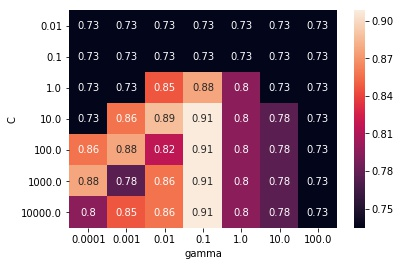
\includegraphics[scale=1]{svms/cv_heatmap.jpg}
\end{center}
The pair with the maximum 5-fold cross validation score on the given training set is $(C = 10,\gamma = 0.1)$ with the score $0.9082$. The radial kernel svm trained on the entire training set $X$ with this pair of hyperparametres obtains an accuracy of $0.9072$ on the test set.

\subsection{Inspecting the kernel expansion}

Unfortunately, I have not had the time to complete this part of the assignment.